\begin{tcolorbox} %makes a white opaque background for the text.
	\part{Introduction}
	\lettrine{S}{istem} Migovec, tucked away at the western edge of the Trigavski Narodni Park is the longest cave system in Slovenia. It has been since 2012, when, defying the expectations after a half a decade of effort, the connection between the ‘Old System’ (M2-M16-M18) and the newer Vrtnarija (Gardener’s World) and Vilinska Jama cave was forged after a routine pushing trip at -600m. This - 38 years since the beginnings of exploration underneath Tolminski Migovec, ‘Mig’ as it is affectionately named - made the national news. 

Since then, and rather more discreetly,  Imperial College cavers (ICCC) have repeatedly spent their summers discovering more voids under the hollow mountain, in tandem with the Jamarska Sekcija Planinskega Drustva Tolmin (JSPDT). Bit by bit, the other pieces of the puzzle were extended and connected to the main system. In October 2015, three Slovene cavers found a way between the last big independent cave system, Primadona-Monatip-Uben571 and one of the earliest high level passages of Sistem Migovec, bringing the total to 35.6km of connected passage. Since October 2017, it stands at 39.2km.
\end{tcolorbox}
	\backgroundsetup{	scale=1,
					color=black,
					opacity=1,
					angle=0,
					contents={%
							  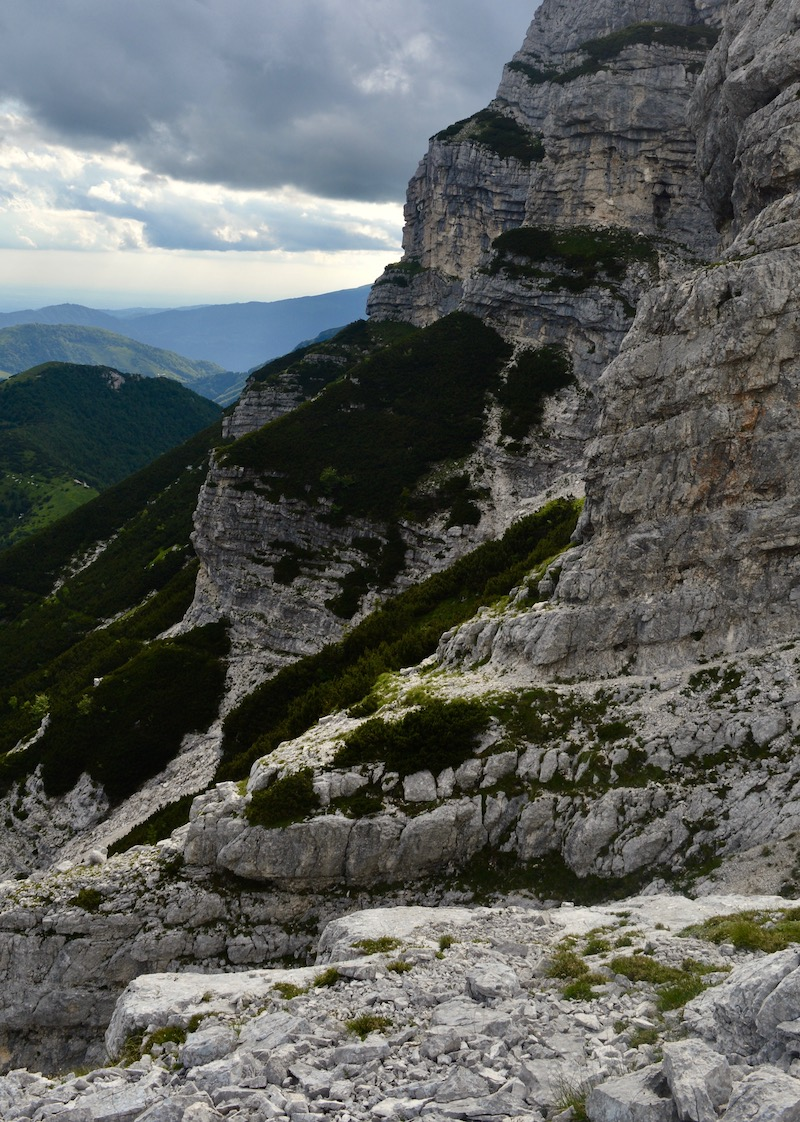
\includegraphics[height=\paperheight]{backgrounds/migface.jpg}
  					} % this puts the entire image as local background
	}
\BgThispage %calls the image to be displayed as background, flush with paper edge.